\chapter{I-Mode Pedestal Stability Modeling}\label{ch:ImodeModeling}

Large, uncontrolled Edge-Localized Modes (ELMs -- see \cref{sec:hcr_elmy}) in ITER-scale operation are expected to drive unacceptable levels of pulsed heat loading and erosion damage to plasma-facing materials \cite{Loarte2003,Federici2003}.  As such, avoiding or mitigating large ELMs is a major focus of research in high-performance regimes: approaches include active ELM control in H-mode (\cref{subsec:hcr_elmy_control}) and inherently ELM-suppressed regimes (\cref{sec:hcr_elmsuppressed}).  To these we add the I-mode (\cref{sec:hcr_imode}), which appears to be naturally stable against large, deleterious ELMs in addition to its other beneficial properties (see \cref{ch:ImodePedestal}).

Confidence in plans for high-performance operation on ITER- and reactor-scale devices requires a predictive model for the pedestal structure and stability, to optimize fusion performance and ELM control or avoidance.  Recent cooperative efforts among theory, modeling, and experiment \cite{Groebner2013} have resulted in such a model for ELMy H-modes, termed EPED \cite{Snyder2009,Snyder2011}, detailed in \cref{sec:mod_eped}.  The EPED model combines constraints from peeling-ballooning MHD stability (\cref{sec:mod_pb}) \cite{Wilson2002,Snyder2004,Wilson2006}\gnote{cites?} and kinetic-ballooning turbulence (\cref{sec:mod_turbulence}) \cite{Snyder1999,Candy2005,Snyder2001}.  The EPED model has been successfully implemented in ELMy H-mode on a number of machines, including DIII-D \cite{Snyder2009,Snyder2011}, JT-60U \cite{Snyder2009}, C-Mod \cite{Walk2012}, and KSTAR \cite{Han2013}, as well as in QH-mode \cite{Snyder2012}; small/no-ELM regimes (EDA H-mode, type-II and type-III ELMy H-modes) have been shown to be 
stable against the drive identified in the EPED model \cite{Snyder2009}.

In this chapter, we apply the EPED approach to I-mode, examining the stability of the I-mode pedestal against peeling-ballooning MHD and kinetic-ballooning turbulence \cite{Walk2014}.  This is compared to the observed lack of large ELMs in I-mode, with a goal of examining the parameter space in which stationary ELM-free operation with I-mode is possible.  We also examine the stability and edge behavior of cases in which small, intermittent ELM-like events are observed in I-mode operation.\nicesectionending

\section{MHD Stability -- ELITE}\label{sec:imode_elite}

The triggering of large ELMs in H-mode has been identified with the interaction between pressure-driven ballooning and current-driven edge kink/peeling MHD instabilities (the latter is typically referred to as a ``peeling'' mode to distinguish it from similarly current-driven core kink modes) in the pedestal \cite{Wilson2002,Snyder2004,Wilson2006}.  Numerical studies of these instabilities using the ELITE code \cite{Wilson2002,Snyder2003}, detailed in \cref{subsec:mod_elite}, have proven quite successful in capturing the physics of the ELM trigger.

\subsection{ELITE Implementation}\label{subsec:imode_elite_setup}

At its simplest, a single pass in ELITE calculates the growth rate of the peeling-ballooning instability at fixed toroidal mode number $n$ for a given plasma profile (to wit, the pressure gradient and current density in the pedestal) and equilibrium \cite{Snyder2013}\gnote{how much of this in ch 3?}.  This requires a reconstructed magnetic equilibrium with sufficiently high point density to capture the rapid variation in flux surfaces near the edge -- all results in this chapter were prepared using high-resolution EFIT \cite{Lao1985} reconstructions constrained by kinetic profiles\gnote{better ref for kinetic EFIT?} -- and high-resolution diagnostics to generate accurate profile measurements in the pedestal.  To fully capture the physics of the pedestal, however, it is beneficial to visualize the pedestal relative to the full stability boundary (see \cref{fig:mod_pbcartoon} for a schematic illustration), typically expressed in terms of the pressure-gradient and current-density drive terms.  

Beginning from the experimental result, the profiles are scaled at fixed pedestal width, such that the pressure pedestal height or peak current density is increased or decreased relative to the original by a scalar factor, after which a self-consistent EFIT reconstruction is attempted.  This effectively fills in a grid in $\alpha_{MHD} - j$ space (a practice commonly termed ``varyped'').  Horizontal slices scaling the pressure pedestal height (and therefore gradient) at fixed current, and vertical slices scaling the current density at fixed $\nabla p$ -- although ELITE does not explicitly distinguish between density and temperature profiles, these slices implicitly vary density and temperature relative to each other (for example, increased bootstrap current at fixed $\nabla p$ in a vertical slice requires increased density and decreased temperature, and vice versa for horizontal slices) \cite{Snyder2013}.  Note that the practice described in \cref{sec:mod_eped} of increasing pressure (and pressure gradient) at fixed width to find the maximum ELM-stable pressure as a function of width is essentially a diagonal slice through the grid: only the pressure profile is explicitly scaled, with the bootstrap current allowed to self-consistently vary\gnote{cite?}, and will increase with increasing $\nabla p$.  At each point in the $\alpha_{MHD} - j$ grid, ELITE is run on a range of mode numbers (here $5 \le n \le 35$) to find the most unstable mode\gnote{note low-$n$ peeling, higher-$n$ ballooning in ch 3} and its growth rate; this is normalized to diamagnetic stabilization effects by the threshold for instability onset, $\gamma_{MHD} > \omega_{*eff}/2$ where $\omega_{*eff}$ is the effective diamagnetic frequency accounting for variation in the pedestal, as implemented in EPED1.6 (see \cref{subsec:mod_eped16}).

\begin{figure}[p]
 \pushtooutside
 \ffigbox[\FBwidth]{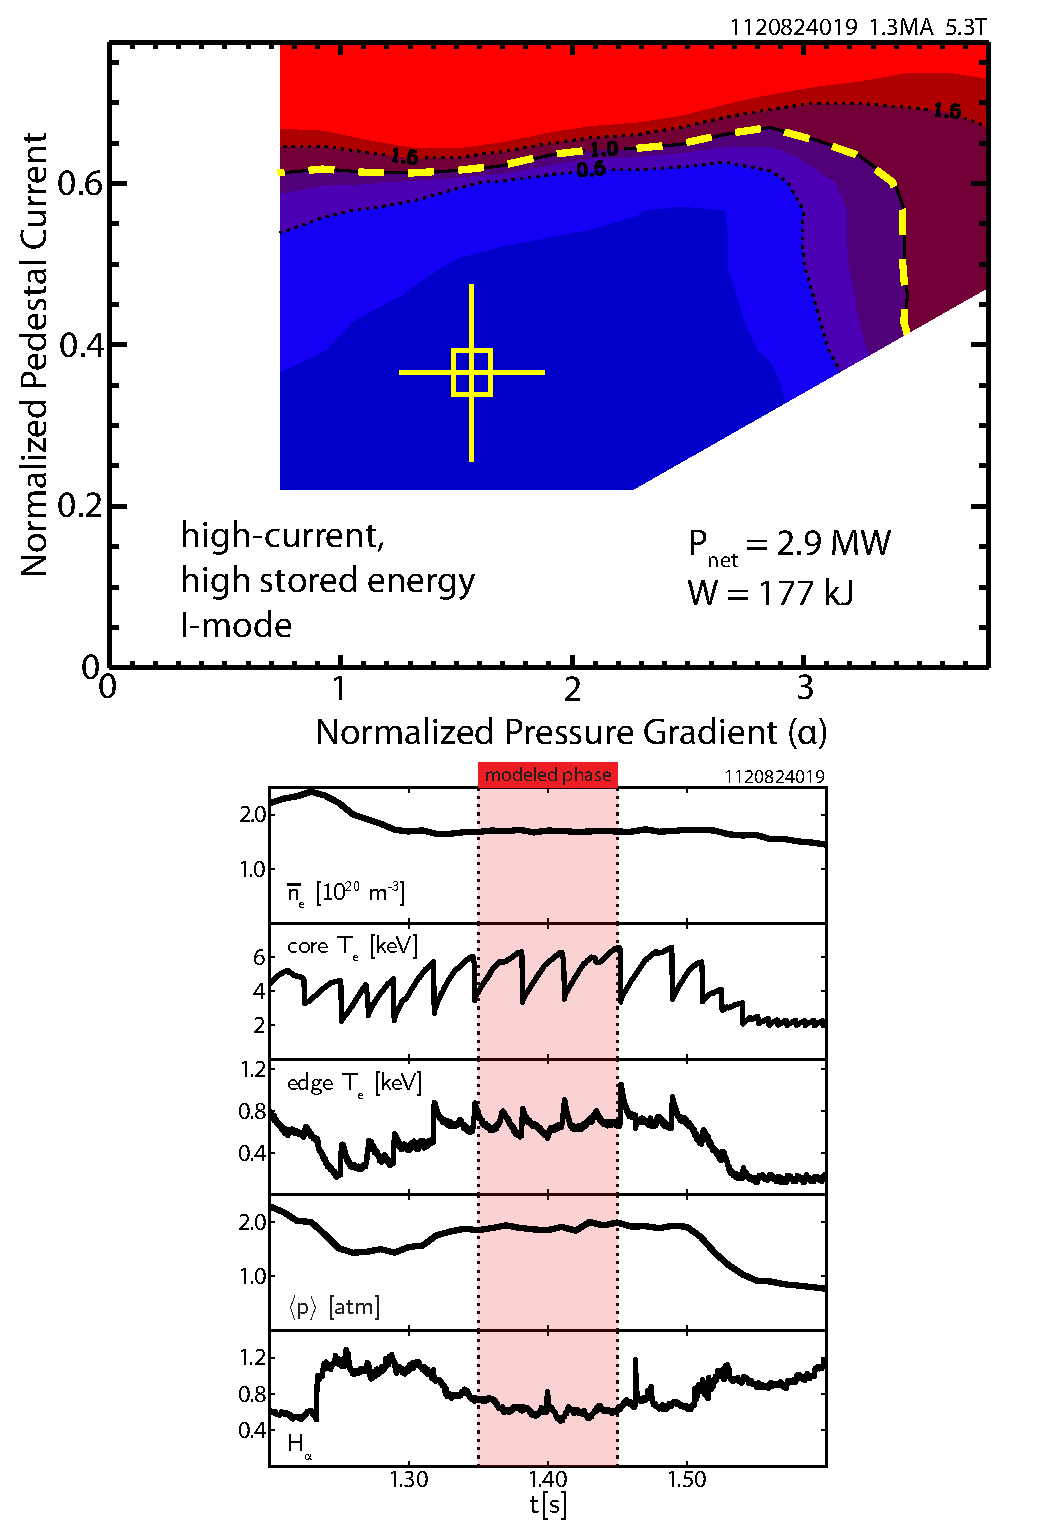
\includegraphics[width=150mm]{graphics/IModeModeling/1120824019_ELITE_stitch_vert.pdf}}{\caption[I-mode pedestal MHD stability contour generated by ELITE.]{MHD stability contour for a high-current ($\SI{1.3}{\mega\ampere}$), high-performance I-mode generated by the ELITE code.  The experimental measurement is shown by the crosshair, with the stability boundary indicated by the yellow dashed line.  Parameters for the modeled phase of the discharge are shown below.  The I-mode pedestal is observed to be far from both the peeling and ballooning MHD stability boundaries.}\label{fig:imode_elite_noelm}}
\end{figure}

\subsection{I-Mode ELITE Calculations}\label{subsec:imode_elite_calc}

An ELITE calculation for the I-mode pedestal is shown in \cref{fig:imode_elite_noelm}, along with parameters (line-averaged density, core and edge $T_e$, global-average pressure, and $H_\alpha$ emission) for the modeled phase of the discharge.  The pedestal, indicated by the yellow crosshair, is far from both the peeling and ballooning MHD stability boundaries calculated by ELITE (indicated by the yellow dashed line, marking the $\gamma/(\omega_{*eff}/2) = 1$ contour).  This is consistent with the observed lack of large ELMs, even in higher-performance I-modes (both in the normalized sense, with $H_{98} = 1.02$ and $\beta_N = 1.0$, and in absolute terms, $W_{MHD} = \SI{177}{\kilo\joule}$ in the case in \cref{fig:imode_elite_noelm}).  The calculated MHD stability is intuitively understood from the I-mode pedestal profile: the lack of a strong density pedestal reduces both the total pressure gradient, reducing the ballooning drive, and the edge current, reducing the peeling drive (recall from \cref{eq:jboot} that $\nabla n_e$ is the dominant term setting the bootstrap current).  A comparison of the pedestal profiles, with pressure gradient and edge current density, between I-mode and H-mode is shown in \cref{fig:imode_elmy_profs}:

\begin{figure}[h]
 \pushtooutside
 \fcapside[60mm]{\caption[Pedestal profiles in I-mode and ELMy H-mode.]{Pedestal profiles in I-mode and ELMy H-mode.  Due to the steep density gradient in the pedestal, the H-mode exhibits significant pressure gradient and edge current density, which drive the peeling-ballooning MHD instability associated with the ELM trigger.  Despite this, the high edge temperature in I-mode allows it to reach an appreciable pedestal pressure.}\label{fig:imode_elmy_profs}}{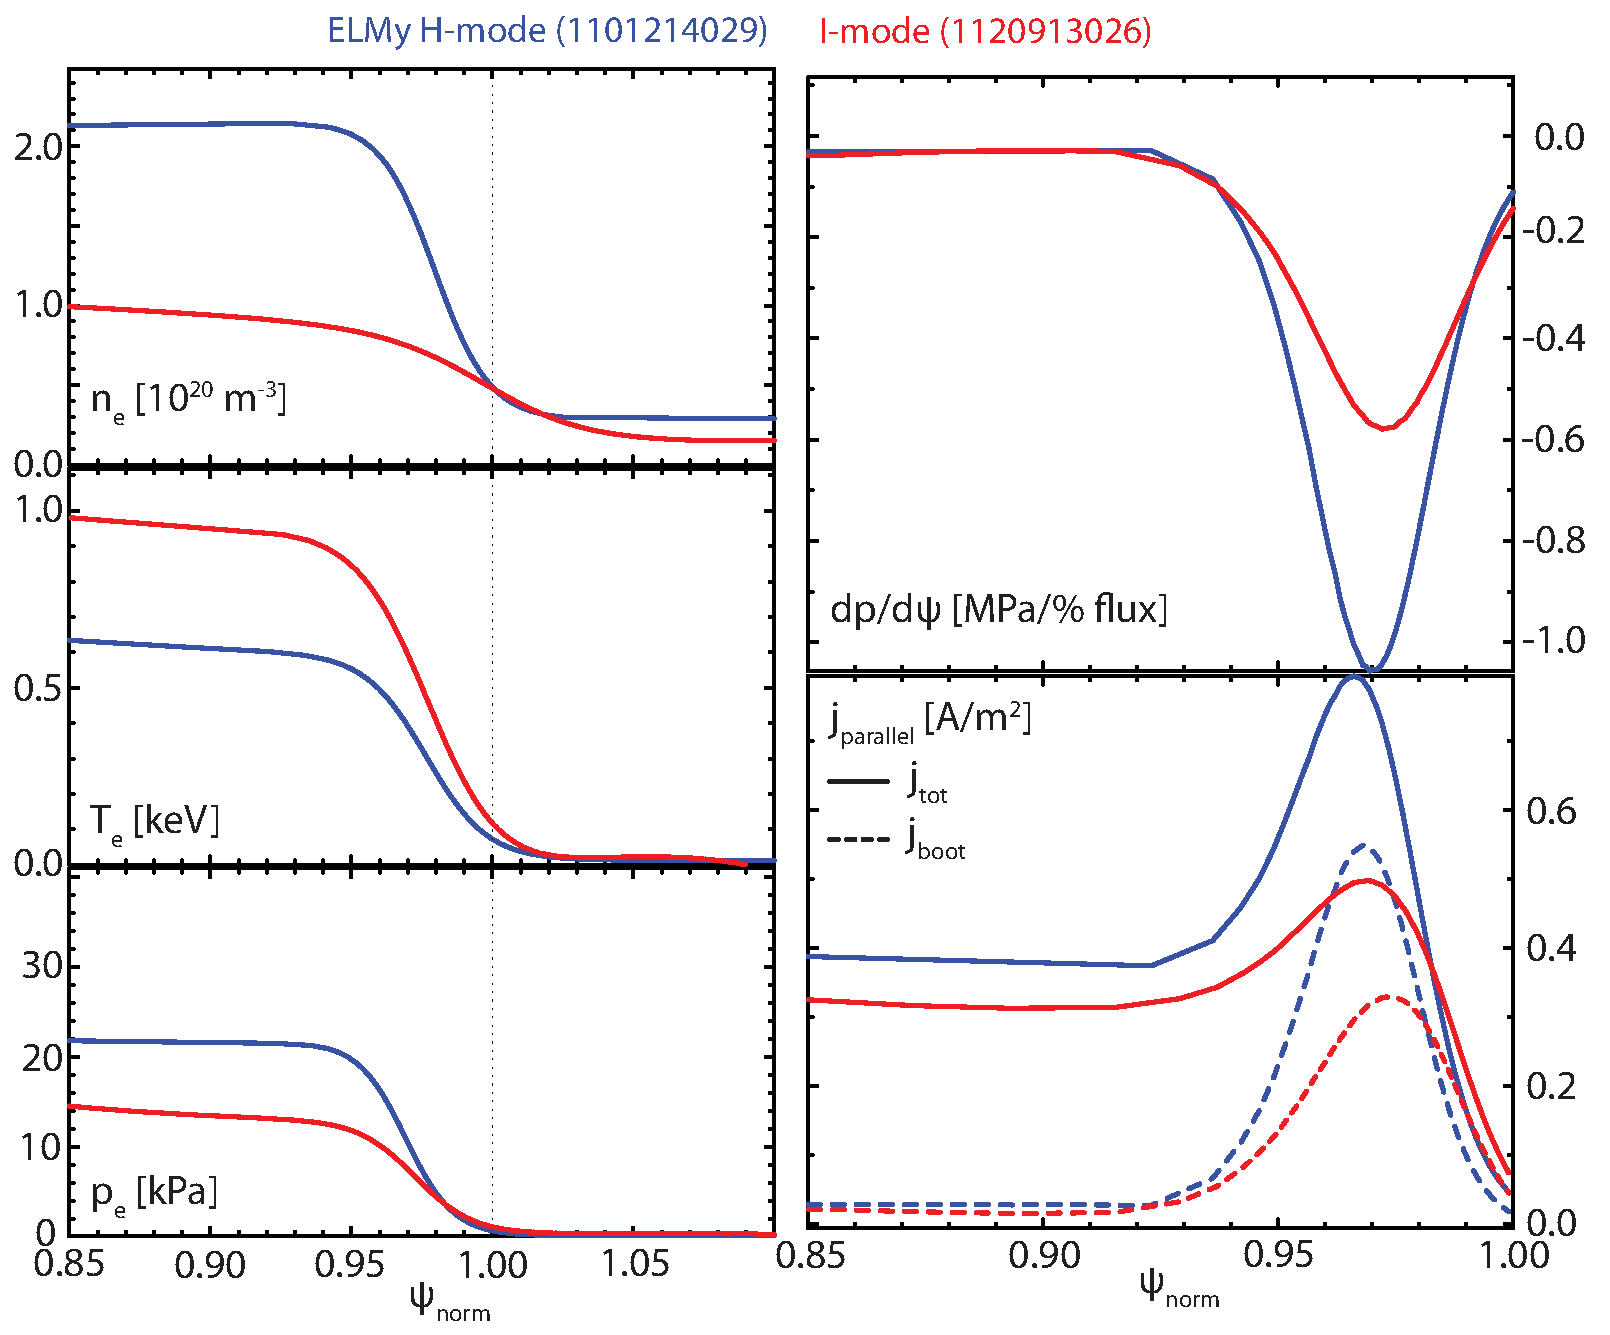
\includegraphics[width=100mm]{graphics/IModeModeling/prof_elmy_imode.pdf}}
\end{figure}

\begin{figure}[p]
 \pushtooutside
 \ffigbox[\FBwidth]{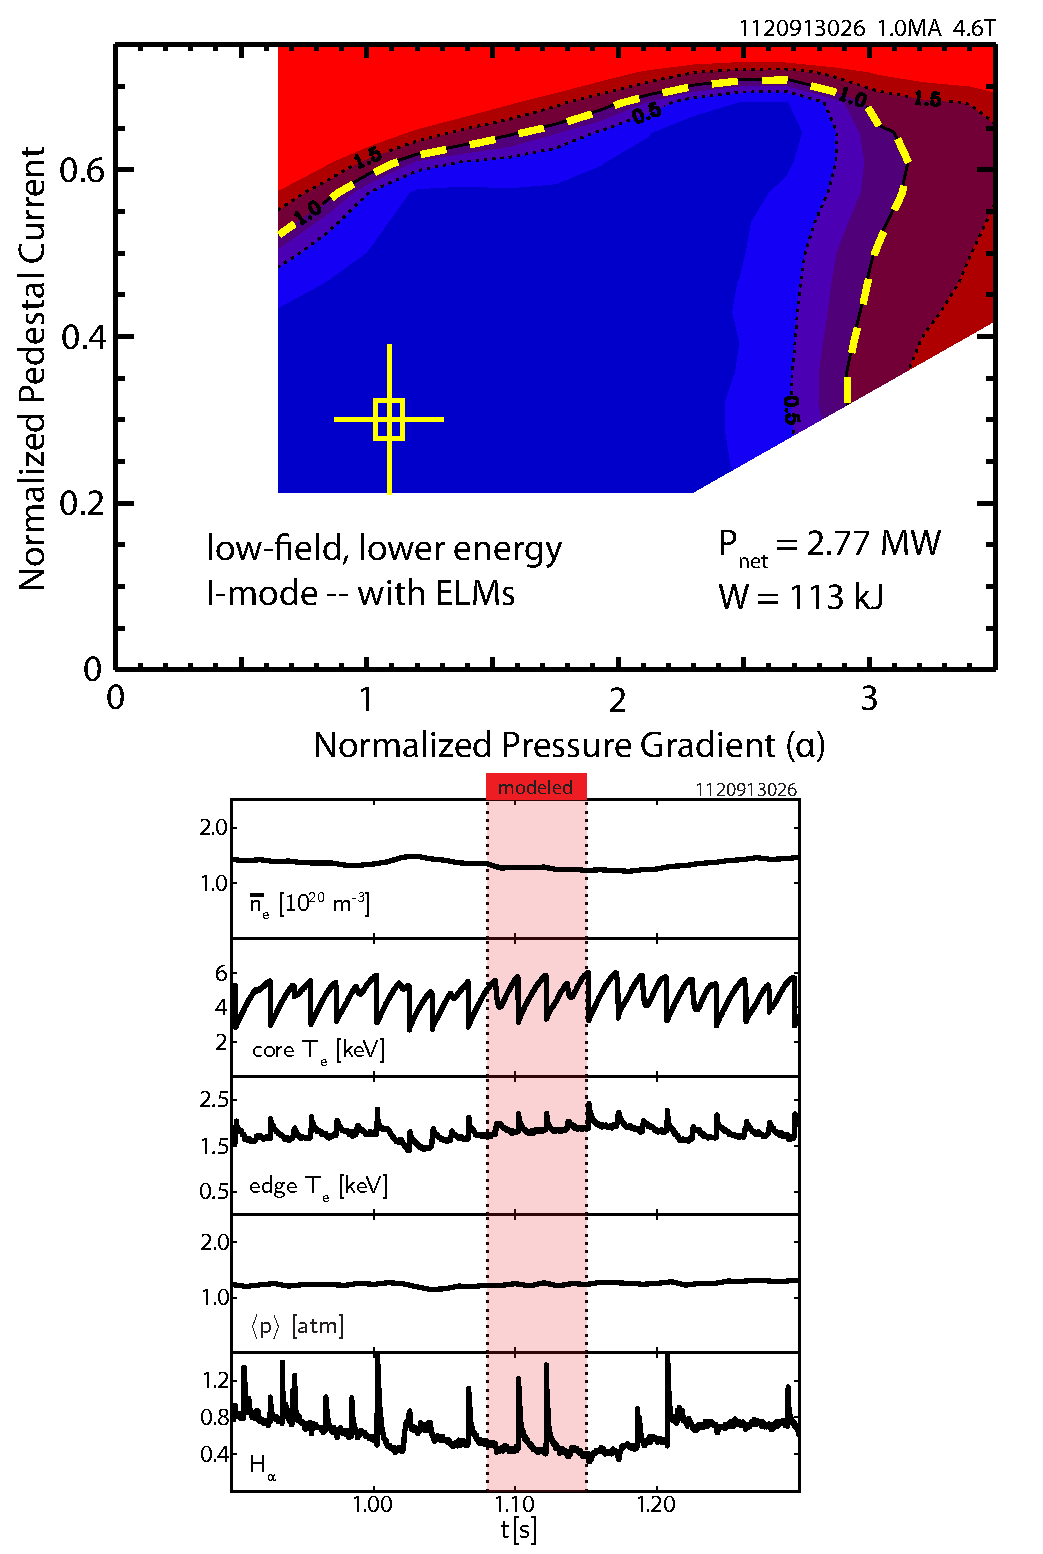
\includegraphics[width=150mm]{graphics/IModeModeling/1120913026_ELITE_stitch_vert.pdf}}{\caption[I-mode pedestal MHD stability contour generated by ELITE -- low-field case exhibiting ELM-like events.]{MHD stability contour for a low-field, lower-energy I-mode generated by the ELITE code.  The experimental measurement is shown by the crosshair, with the stability boundary indicated by the yellow dashed line.  Parameters for the modeled phase of the discharge are shown below.  This case exhibited small,intermittent ELM-like events, but is still calculated to be peeling-ballooning stable.}\label{fig:imode_elite_stelm}}
\end{figure}

Although I-mode is free of the regular, large ELMs typical of (type-I) ELMy H-mode, under certain conditions -- particularly reduced toroidal field and plasma current -- small ($<1\%$ drop in stored energy) intermittent ELM-like events are occasionally observed in I-mode.  However, when examined in ELITE (\cref{fig:imode_elite_stelm}) these cases are found to still be far from the peeling-ballooning boundary.  These intermittent events occur in conjunction to sawtooth heat pulses reaching the edge, visible on the fast ECE $T_e$ signal, indicating that the events are potentially triggered by transient modification of the pedestal by the heat pulse -- however, these events are not consistently triggered on each sawtooth crash under similar conditions.  More study is required on this front, with initial results shown in \cref{sec:imode_elms}.\gnote{move this to later section?}

\begin{figure}[t]
 \pushtooutside
 \ffigbox[\FBwidth]{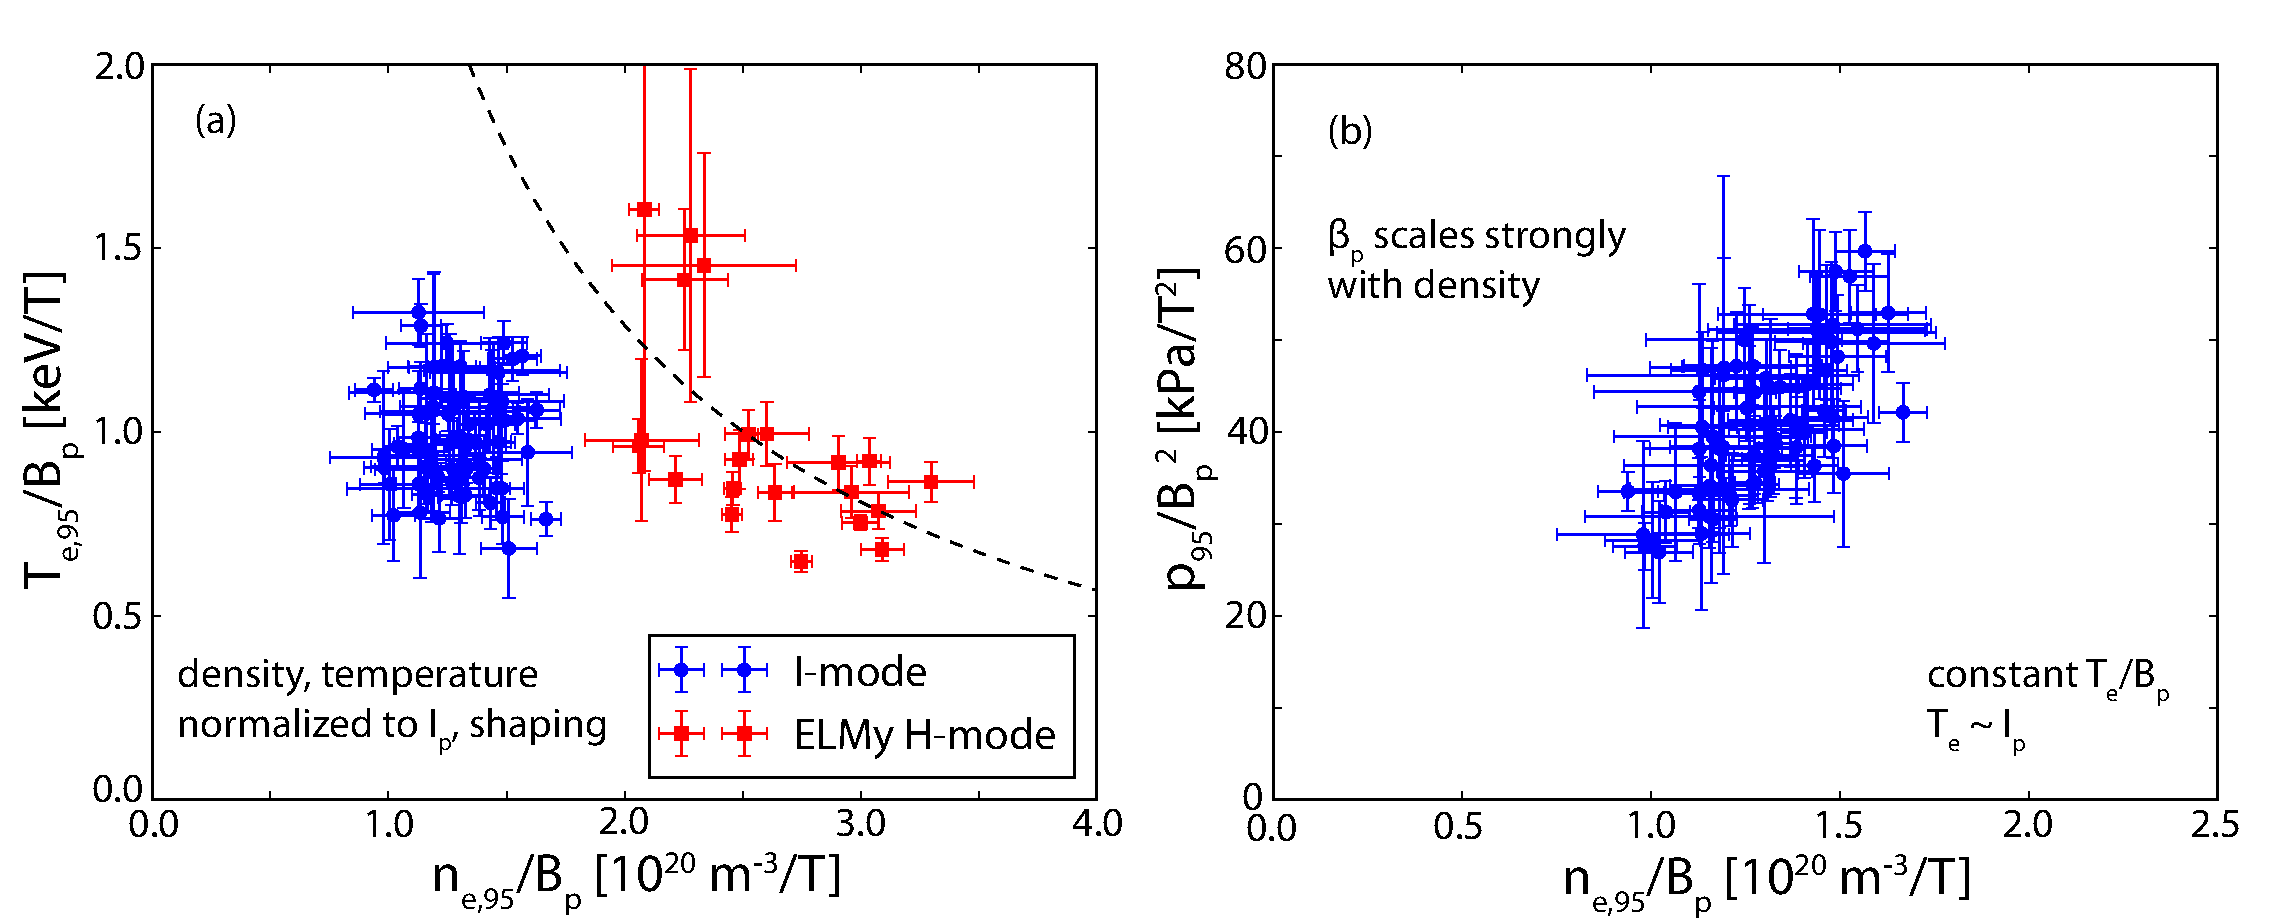
\includegraphics[width=150mm]{graphics/IModeModeling/neBp_stitch.pdf}}{\caption[Normalized pedestal temperature and pressure versus density.]{Pedestal temperature (left) and pressure (right) versus pedestal density.  Parameters are normalized to the edge poloidal field -- this accounts for plasma-current variation in the datapoints, as well as allowing a natural representation of MHD boundaries.  (a) Pedestal temperature vs. density for I-mode and ELMy H-mode.  Due to the poloidal-field normalization, hyperbolae in the parameter space are curves of constant $\beta_{p,ped}$.  ELMy H-modes lie, to lowest-order approximation, on a $\beta_{p,ped}$-limited curve (indicated by the dashed line) with the expected inverse relationship between density and temperature; I-mode $n_e$ and $T_e$, however, are uncorrelated.  (b) Normalized pedestal pressure versus density in I-mode.  Pedestal poloidal beta trends linearly with (normalized) density, rather than lying on the $\beta_{p,ped}$-limited line 
expected for MHD-limited pedestals, consistent with the strong response of the I-mode pedestal to fueling (see \cref{subsec:imode_fueling}).  I-mode data lie on a line of constant $T_e/B_p$, consistent with the observed $T_{e,ped} \sim I_p$ seen in \cref{subsec:imode_temp}.}\label{fig:neBp_stitch}}
\end{figure}

Examination of the I-mode pedestal is also illuminating from the perspective of MHD stability.  To lowest order approximation, MHD-limited pedestals, as are found in ELMy H-mode, are limited in the attainable poloidal beta at the pedestal top (a limit arising from the limit on $\alpha_{MHD}$ from ballooning instability coupled with the weakly-varying pedestal width on a given tokamak -- \cf \cref{subsec:hcr_elmy_fluct}).  This is illustrated in \cref{fig:neBp_stitch}(a), showing the pedestal density and temperature normalized to poloidal field (accounting for variation in plasma current).  Due to the normalization to $B_p$, hyperbolae in the parameter space are curves of constant pedestal $\beta_{p}$.  ELMy H-mode data lie on such a curve (note that, since the $\beta_p$ limit is shaping-dependent, only ELMy H-mode cases with approximately matched shape are shown on the single hyperbolic curve)\gnote{footnote this?}, with the expected inverse relationship between pedestal density and temperature.  I-mode pedestal density and temperature, on the other hand, are uncorrelated, consistent with the pedestal not being limited by MHD stability constraints.  I-mode pedestal pressure, similarly normalized, is shown against normalized pedestal density in \cref{fig:neBp_stitch}(b).  Where MHD-limited pedestals would show a flat trend due to the limit on poloidal beta, I-mode $\beta_p$ instead exhibits a linear trend with density.  This is consistent with the strong response of pedestal performance with increased fueling (described in \cref{ch:ImodePedestal}, particularly \cref{subsec:imode_fueling}) provided sufficient heating power to maintain the pedestal.  The slope of this trend is a line of constant $T_{e,95}/B_p$, consistent with the observed $T_e \sim I_p$ as well (see \cref{subsec:imode_temp}).\nicesectionending

\section{Kinetic-Ballooning Mode Stability}\label{sec:imode_baloo}

\begin{figure}[t]
 \pushtooutside
 \ffigbox[\FBwidth]{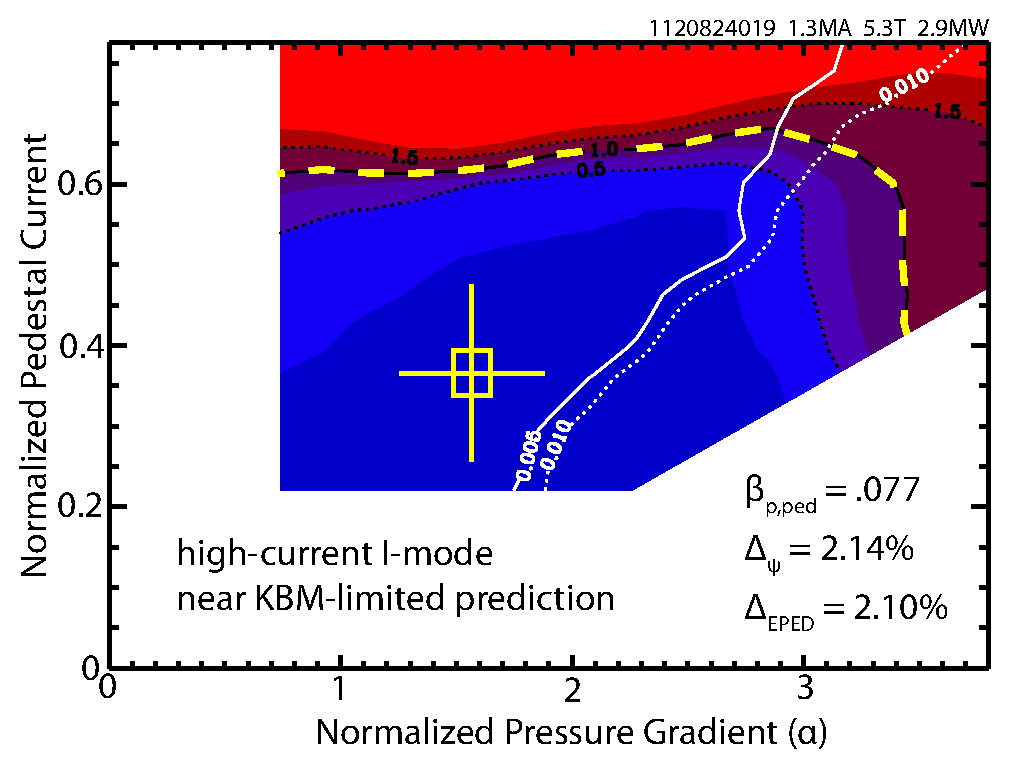
\includegraphics[width=150mm]{graphics/IModeModeling/1120824019_1400n5_35_gamws16_bal.pdf}}{\caption[Infinite-$n$ ballooning MHD prediction, overlaid on ELITE result (\cref{fig:imode_elite_noelm}).]{Infinite-$n$ ballooning MHD results calculated by BALOO, overlaid on the ELITE results for the same case (see \cref{fig:imode_elite_noelm}).  The Infinite-$n$ ballooning threshold is taken as a surrogate for the onset of KBM turbulence.  Due to the local nature of the infinite-$n$ constraint, BALOO calculates the width in flux space that is locally ballooning-critical -- when this reaches half of the pedestal width, the KBM is triggered.  This case is near the KBM-predicted pedestal width $\Delta_{EPED}$, but is nevertheless modeled to be KBM-stable (for $\Delta_\psi \sim 0.02$, the half-width threshold is the $0.01$ contour).}\label{fig:imode_baloo_noelm}}
\end{figure}

\begin{figure}[t]
 \pushtooutside
 \ffigbox[\FBwidth]{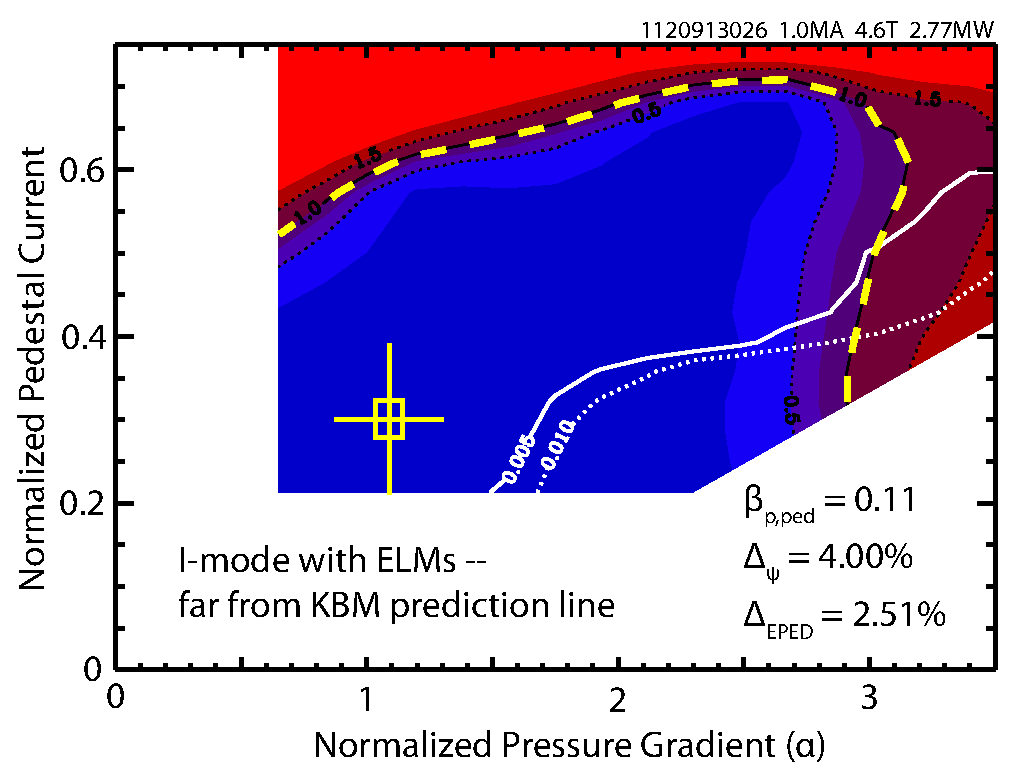
\includegraphics[width=150mm]{graphics/IModeModeling/1120913026_1186n5_35_bal_jalpha.pdf}}{\caption[Infinite-$n$ ballooning MHD prediction, overlaid on ELITE result (\cref{fig:imode_elite_stelm}).]{Infinite-$n$ ballooning MHD results calculated by BALOO, overlaid on the ELITE results for the same case (see \cref{fig:imode_elite_stelm}).  This case exhibited sawtooth-triggered ELM-like events.  This case is substantially wider than the KBM-predicted pedestal width $\Delta_{EPED}$, and is modeled to be strongly KBM-stable -- in fact, the BALOO assay could not calculate enough ballooning-unstable rational surfaces to draw the contour for the BCP-predicted threshold of $0.02$.}\label{fig:imode_baloo_stelm}}
\end{figure}

Edge turbulence in I-mode is characterized by the strong reduction of mid-frequency turbulence corresponding to the reduced energy transport after the L-I transition\gnote{reword?}.  In its place, the I-mode pedestal exhibits a broad higher-frequency ($200-400\;\si{\kilo\hertz}$) fluctuation, the \emph{Weakly-Coherent Mode} \cite{Whyte2010,Hubbard2011,Cziegler2013} (see \cref{subsec:hcr_imode_wcm}).  Due to its prominence in the I-mode edge and functional similarity to the Quasi-Coherent Mode (QCM) in EDA H-mode \cite{Hubbard2001} (see \cref{subsec:hcr_eda}), the WCM is thought to play a role in regulating the I-mode pedestal, particularly by driving enhanced particle flux \cite{Dominguez2012}.  While the WCM is fairly well-characterized experimentally, the underlying physics of the mode remain an open question.  From the standpoint of both turbulence characterization and ELM stability, the kinetic-ballooning mode (KBM) is a valuable starting point for comparing the WCM to the turbulent behavior in more conventional H-modes.\gnote{reword?}

Computational modeling of the KBM is possible using infinite-$n$ ideal ballooning MHD as a surrogate for the turbulence threshold \cite{Snyder2001,Candy2005,Snyder2009} (see \cref{sec:mod_turbulence}).  The localized constraint from the KBM (and perfectly-localized infinite-$n$ ideal MHD) is applied to the entire pedestal via the ``ballooning-critical pedestal'' technique, described in \cref{subsec:mod_bcp}, in which the KBM threshold is identified as the point at which half of the pedestal (typically the ``middle half'' where the pressure gradient is steepest) is locally at or beyond criticality to the MHD surrogate.  This is calculated using the BALOO code \cite{Connor1979,Miller1987}; at each point in the varyped grid, the number of rational surfaces that are unstable to infinite-$n$ ballooning modes and subsequently the width in poloidal flux space covered by these surfaces is calculated, drawing contours of pedestal half-width corresponding to the KBM threshold.

I-mode pedestals exhibit little trend in width (in poloidal flux space) with pedestal poloidal beta (see \cref{fig:imode_wid_betapol}), as is expected for pedestals limited by KBM turbulence.  We may compare cases spanning the range in pedestal width $\Delta_\psi$ against the KBM-limited prediction for the width, $\Delta_\psi = 0.076 \beta_{p,ped}^{1/2}$, from EPED1 (see \cref{subsec:mod_eped1}), herein termed $\Delta_{EPED}$.  The case near the EPED1 prediction line is shown in \cref{fig:imode_baloo_noelm} (overlaid on the ELITE result for the same case, \cref{fig:imode_elite_noelm}).  For $\Delta_\psi = .021$, the expected KBM threshold based on the BCP half-width calculation is the $0.01$ contour -- the pedestal is calculated to be stable compared to this threshold.  The case far from the EPED1 prediction line is shown in \cref{fig:imode_baloo_stelm} (overlaid on the ELITE result for the same case, \cref{fig:imode_elite_stelm}).  At $\Delta_\psi = 0.04$, the expected KBM threshold is the $0.02$ contour -- however, the BALOO assay could not calculate enough ballooning-unstable rational surfaces to even draw this contour.  Suffice to say that the pedestal is far from the KBM onset threshold as calculated from infinite-$n$ MHD.  Notably, the former case ($\Delta_\psi \sim \Delta_{EPED}$) was a relatively high-performance case, and did not exhibit ELM-like events, while the latter ($\Delta_\psi \gg \Delta_{EPED}$) exhibited ELM-like events.  The indication from both experimental observation and computational modeling, then, is that the KBM is not responsible for limiting the pedestal in I-mode.\nicesectionending

\section{Intermittent ELMs in I-Mode}\label{sec:imode_elms}

Given the importance of controlling or avoiding large ELMs on ITER- and reactor-scale devices, a firm understanding of the physics underlying the ELM trigger is essential for planned ITER operation.  While I-mode is typically observed to be naturally free of large, damaging ELMs, there are nevertheless cases in which small, intermittent ELMs (or ELM-like events) are observed.  It is to these cases that we now turn our attention.

\begin{figure}[p]
 \pushtooutside
 \ffigbox[\FBwidth]{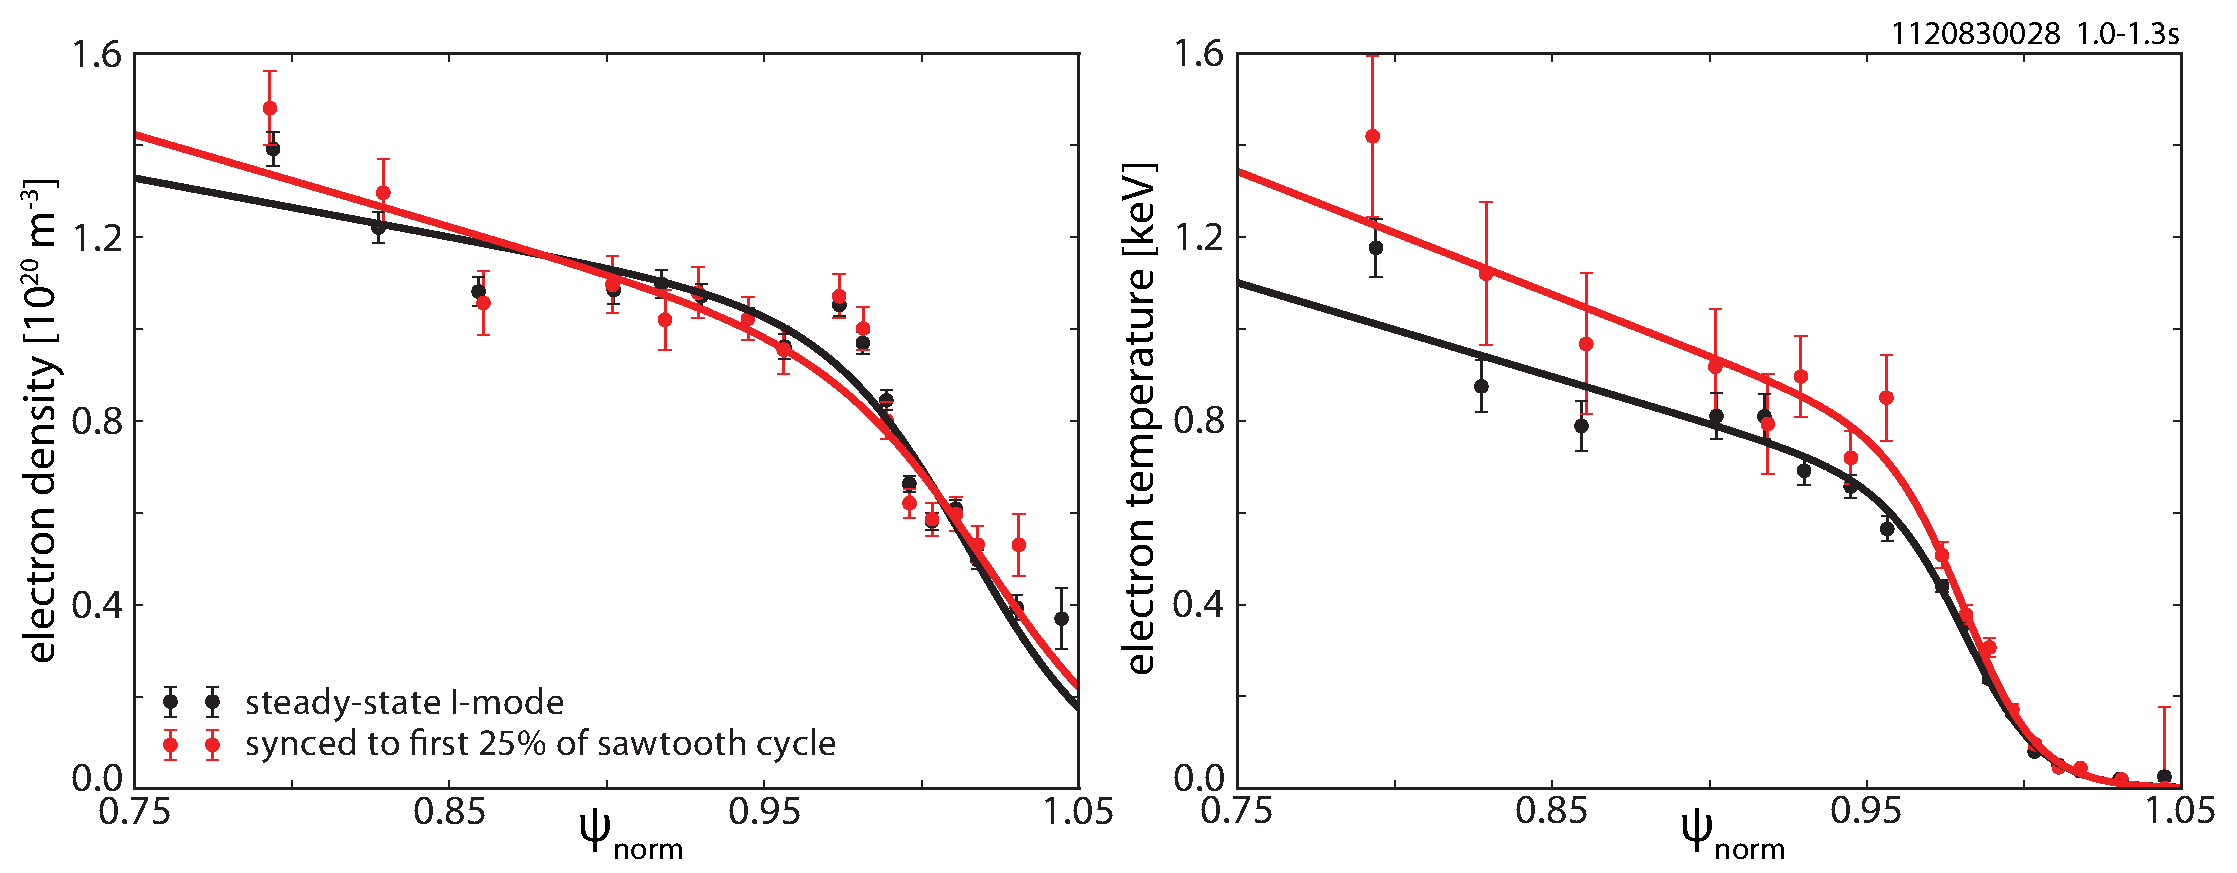
\includegraphics[width=150mm]{graphics/IModeModeling/1120830028_prof_stbin.pdf}}{\caption[Density and temperature profiles in I-mode, showing the modification of the temperature pedestal by the sawtooth heat pulse.]{Profiles of $n_e$ and $T_e$ in the I-mode pedestal, with the full ensemble-averaged data (black) compared to data masked to the first 25\% of the sawtooth cycle following the heat pulse reaching the edge.  The Sawtooth does not meaningfully perturb the density profile, but triggers a measurable transient increase in the temperature pedestal.}\label{fig:prof_stbin}}
\end{figure}

\begin{figure}[p]
 \pushtooutside
 \ffigbox[\FBwidth]{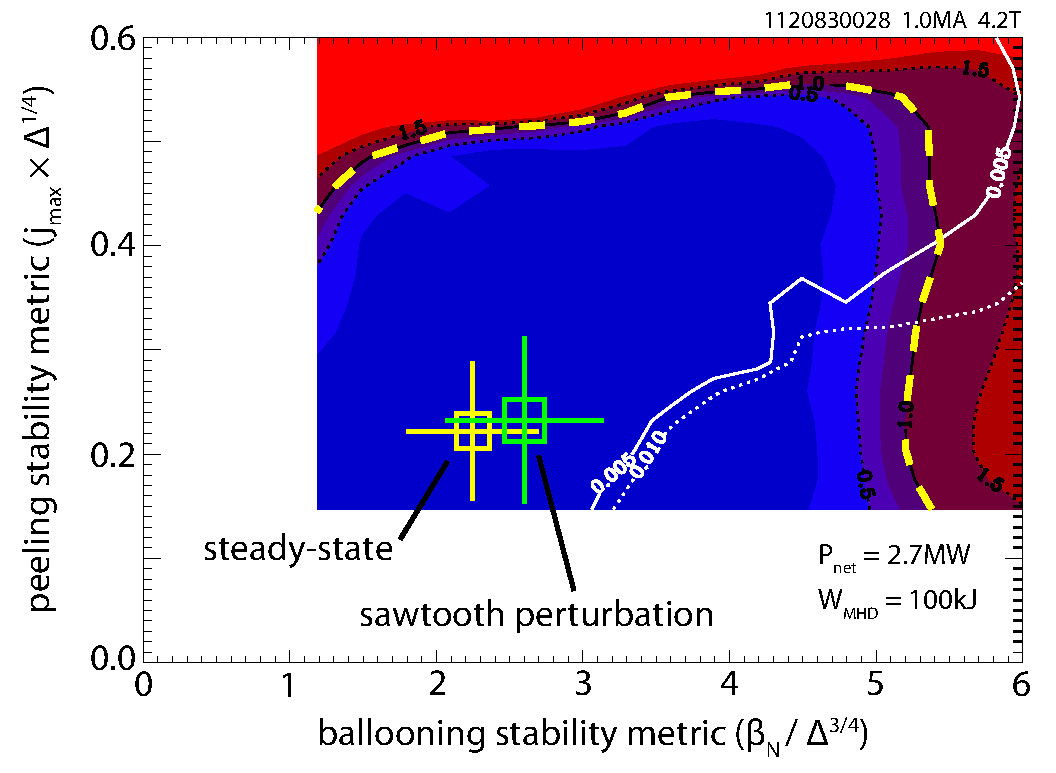
\includegraphics[width=150mm]{graphics/IModeModeling/1120830028_stbin_elite.pdf}}{\caption[Peeling-ballooning MHD and KBM stability in I-mode, showing modification by sawtooth heat pulse.]{Peeling-ballooning MHD stability calculated by ELITE and KBM thresholds calculated by BALOO for an I-mode case, comparing the time-averaged data against pedestal profiles prepared with data masking to the first 25\% of the sawtooth cycle following the heat pulse reaching the edge (see \cref{fig:prof_stbin}).  Note that, to directly compare two separately-calculated equilibria, we replace the $\alpha_{MHD}$ and $j_\parallel$ axes with stability metrics arising from peeling and ballooning MHD.  While the sawtooth heat pulse does measureably perturb the pedestal in stability space, it is insufficient to reach either the peeling-ballooning or KBM threshold.}\label{fig:imode_stbin}}
\end{figure}

ELMs in I-mode are generally observed to be small ($<1\%$ perturbation to the stored energy), and are sporadic, rather than occurring in a regular cycle as in the canonical type-I ELMy H-mode.  These events occur shortly following the sawtooth heat pulse reaching the edge, based on timing from fast ECE $T_e$ measurements in the pedestal.  This indicates a possible trigger for the event due to transient modification of the pedestal structure.  An example case of this is shown in \cref{fig:prof_stbin}.  The sawtooth heat pulse does not perturb the density profile, but drives a significant transient increase in the temperature pedestal (data masked to the first 25\% of the sawtooth cycle after the heat pulse reaches the edge shown in red).  Calculations in ELITE and BALOO for this case are shown in \cref{fig:imode_stbin} for both the time-averaged pedestal profile, and the masked data to the sawtooth cycle.  While the sawtooth synchronization does drive a measurable perturbation to the pedestal in stability space -- the effect is predominantly in the pressure gradient, rather than the current density, due to the weaker effect of the temperature gradient on the bootstrap current -- the effect is insufficient to reach either the peeling-ballooning MHD or the KBM turbulence threshold.  Note that, in order to compare two separately-computed equilibria, we use alternate axes in \cref{fig:imode_stbin}: rather than directly using $\alpha_{MHD}$ and the (normalized) edge current density, the parameter space is presented in terms of ballooning and kink-peeling stability parameters, $\beta_N/\Delta^{3/4}$ and $j_{max} \Delta^{1/4}$.  The first encapsulates the $p_{ped} \sim \Delta^{3/4}$ trend expected from ballooning stability, when accounting for the nonlocal effects -- at broader $\Delta$, wider low-$n$ modes destabilize more easily, reducing the maximum $\alpha_{MHD}$, as described in \cref{sec:mod_pb} -- and current stabilization.  The second accounts for the trend in the total current, $\int j \;d\psi \sim \Delta^{3/4}$\gnote{elaborate in ch 3}; however, the maximum current density and total pedestal current may be related by $\int j \; d\psi \sim j_{max} \Delta \rightarrow j_{max} \sim 1/\Delta^{1/4}$, thus the current-driven kink/peeling stability may be expressed in terms of the normalized $j_{max} \Delta^{1/4}$.

In light of the observed stability of I-mode to peeling-ballooning MHD -- even in cases where the perturbation of the putative sawtooth trigger for ELMs is accounted for -- it is worthwhile to examine the behavior of the ELMs in I-mode compared to those found in more conventional H-modes.  Traces from a type-I ELMy H-mode and an I-mode are shown in \cref{fig:trace_elmy_imode}.  The ELMy case (left) exhibits behavior typical of a type-I ELM cycle: discrete, regular ELMs (visible on the $H_\alpha$) trace, independent of the sawtooth cycle,

\begin{figure}
 \pushtooutside
 \ffigbox[\FBwidth]{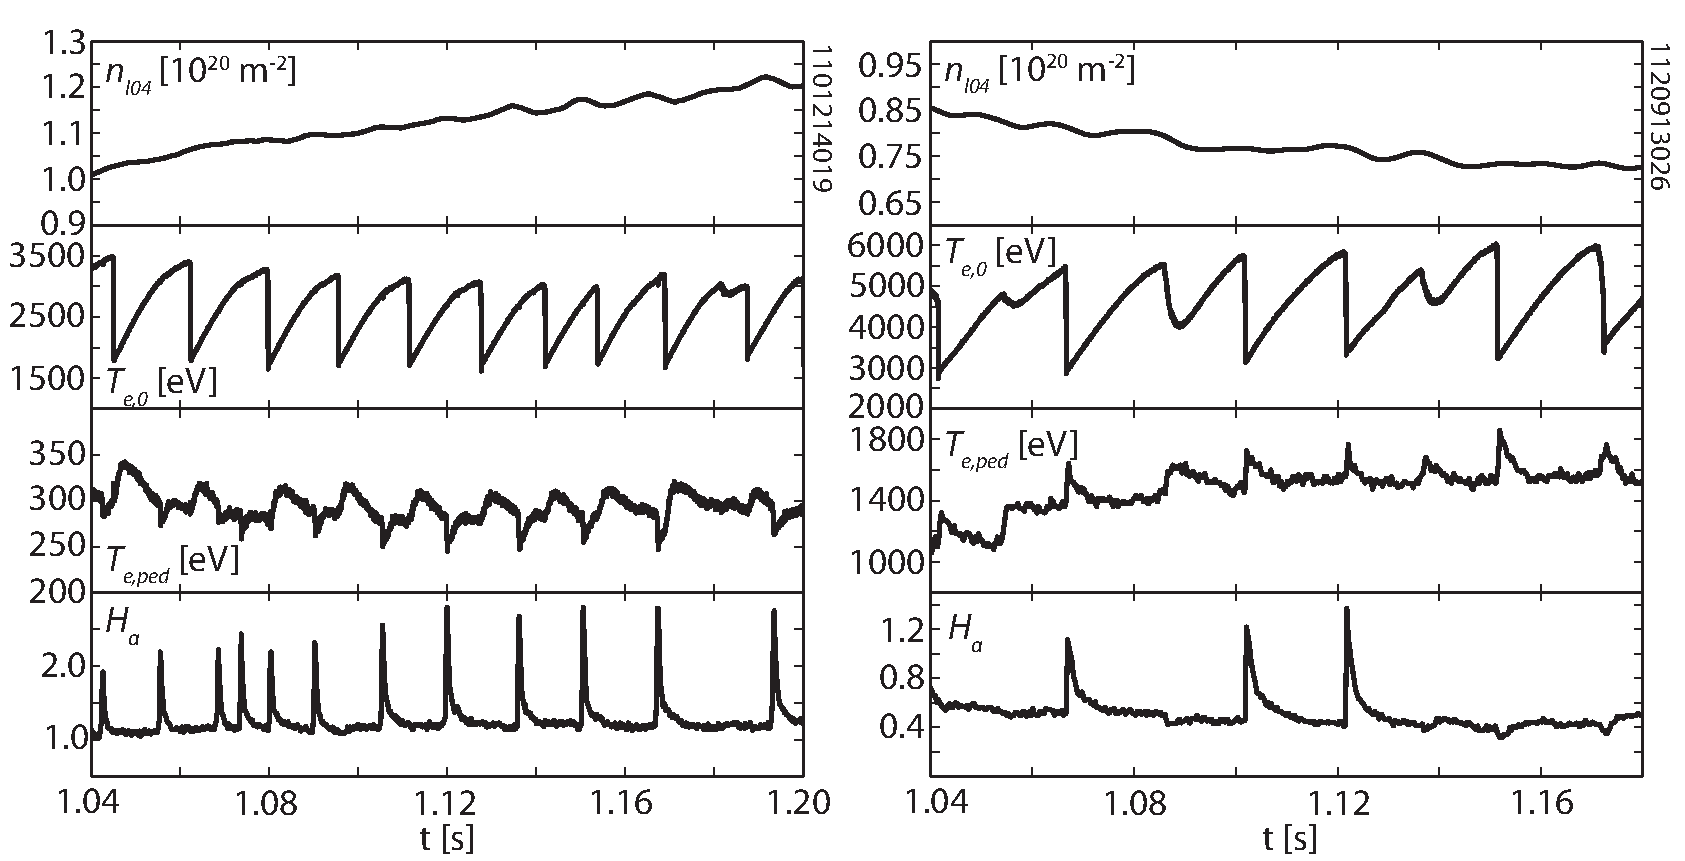
\includegraphics[width=150mm]{graphics/IModeModeling/trace_elmy_imode.pdf}}{\caption[ELM traces for H-mode and I-mode.]{Traces of $n_{l04}$, core and edge $T_e$, and $H_\alpha$ for ELMy H-mode (left) and I-mode (right).  ELMs in H-mode (visible on the $H_\alpha$ trace) are independent of the sawtooth cycle, and drive perturbations to the edge temperature and line-integrated density\note{(?)}, as both energy and particles are expelled form the plasma by the ELM crash.  This is particularly clear on the edge temperature, which exhibits a clear increase with the sawtooth heat pulse and a separate crash with the ELM.  I-mode, in contrast, exhibits ELMs (or ELM-like events) that are tied to sawtooth heat pulses reaching the edge, as visible on the ECE $T_e$ signal.  No visible crash in edge temperature is visible following the ELM, nor is there a significant perturbation to the density\note{(?)}.}\label{fig:trace_elmy_imode}}
\end{figure}

\begin{figure}
 \pushtooutside
 \fcapside[60mm]{\caption[I-mode with a brief H-mode terminated by an ELM, as well as sawtooth-triggered ELM-like events.]{Traces of $n_{l04}$, core and edge $T_e$, and $H_\alpha$ for an I-mode exhibiting ELM-like events.  The sawtooth heat pulse at $\sim \SI{0.87}{\second}$ triggers an I-H transition, indicated by the drop in $H_\alpha$ and suppression of turbulence visible on the $\tilde{n}_e$ plot.  This H-mode terminates with a non-sawtooth-triggered ELM with visible edge temperature crash and density perturbation\note{(?)}, dropping back into I-mode.  The I-mode phase also exhibits sawtooth-triggered ELM-like events with no visible density\note{(?)} perturbation or temperature crash.}\label{fig:trace_imode_welms}}{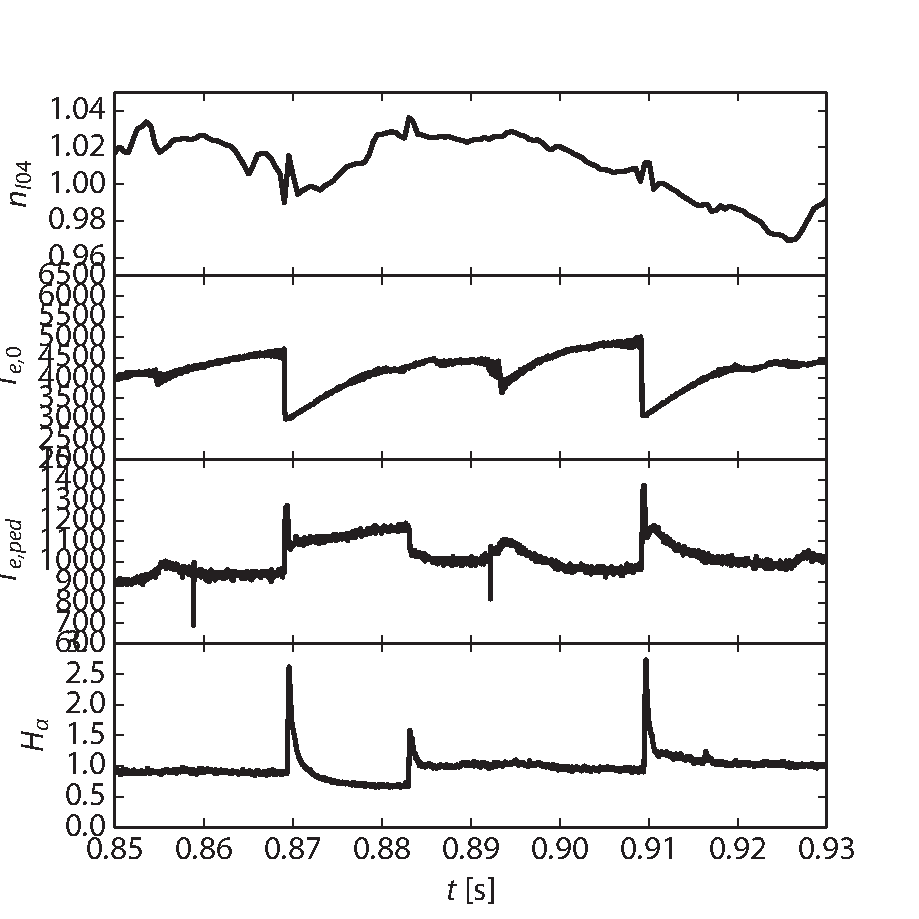
\includegraphics[width=100mm]{graphics/IModeModeling/trace_imode_welms_2.pdf}}
\end{figure}

\begin{figure}[p]
 \pushtooutside
 \ffigbox[\FBwidth]{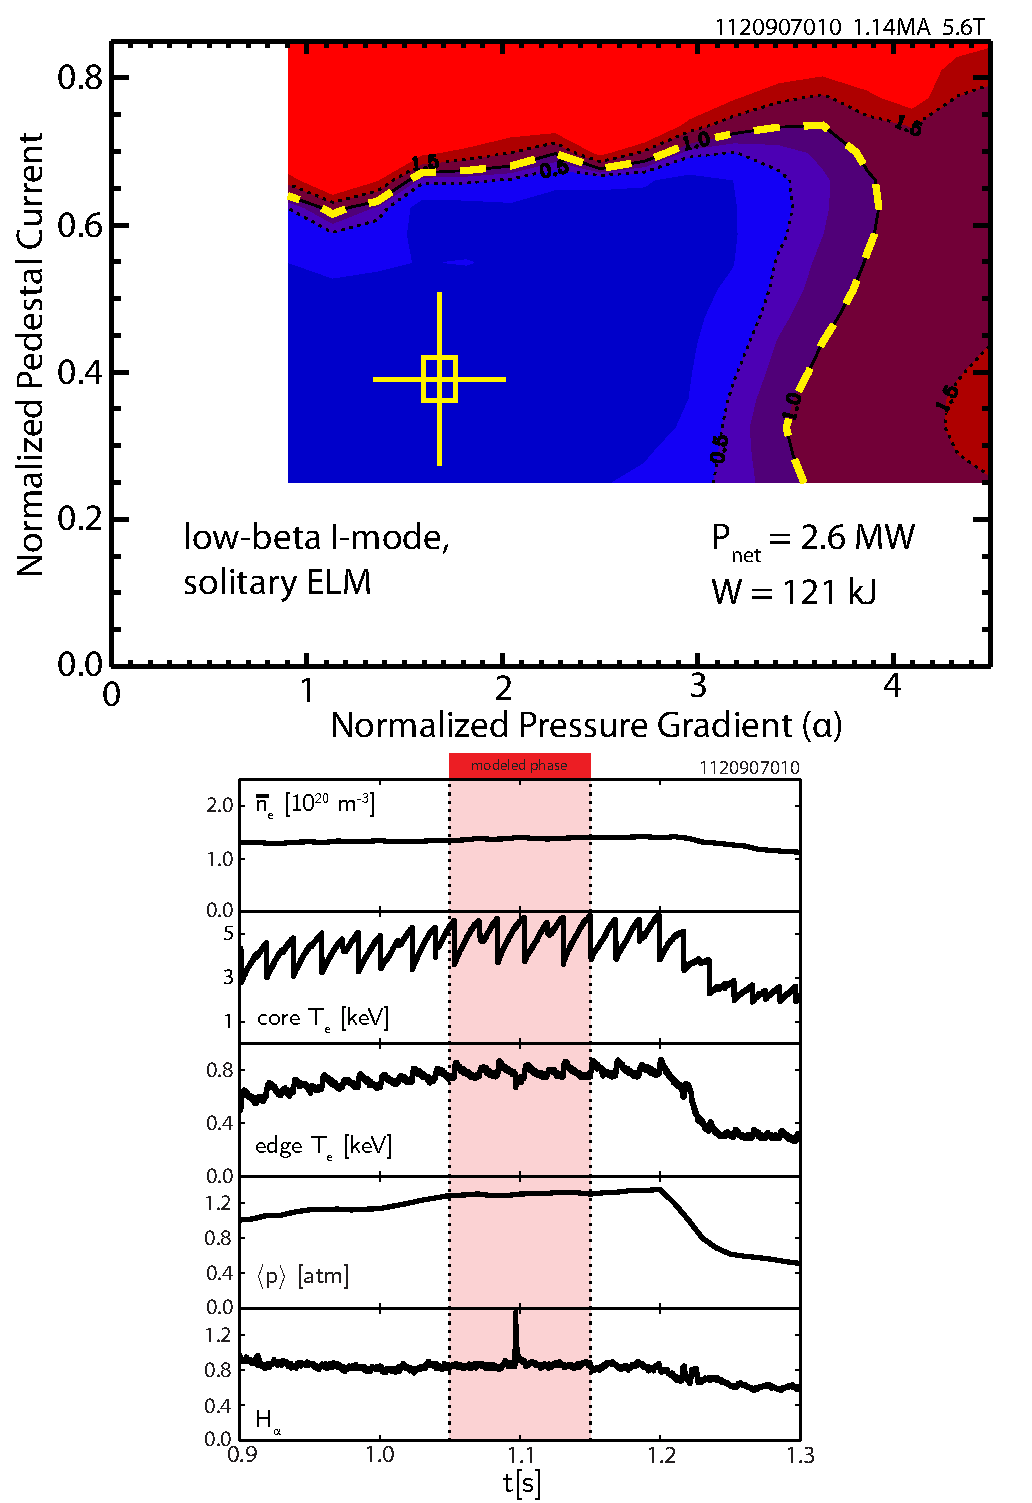
\includegraphics[width=150mm]{graphics/IModeModeling/1120907010_ELITE_stitch_vert.pdf}}{\caption[I-mode pedestal stability contour generated by ELITE -- case exhibiting a non-sawtooth-triggered ELM]{MHD stability contour for I-mode generated by the ELITE code.  The experimental measurement is shown by the crosshair, with the stability boundary indicated by the yellow dashed line.  Parameters for the modeled phase of the discharge are shown below.  This case exhibited a solitary ELM not triggered by the sawtooth heat pulse, with the characteristic edge temperature crash of a canonical ELM.  However, the I-mode phase around the ELM is calculated to be peeling-ballooning stable.  }\label{fig:imode_elite_nonstelms}}
\end{figure}

\begin{figure}
 \pushtooutside
 \ffigbox[\FBwidth]{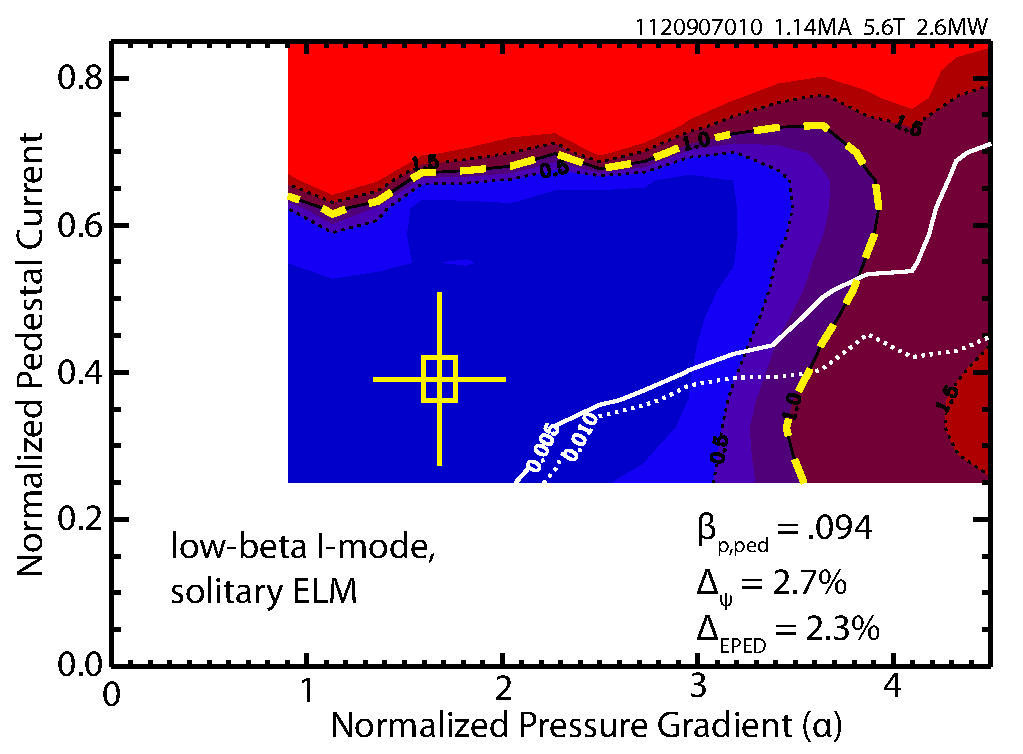
\includegraphics[width=150mm]{graphics/IModeModeling/1120907010_1100n5_35_gamws16_bal.pdf}}{\caption[Infinite-$n$ balooning MHD prediction, overlaid on ELITE result (\cref{fig:imode_elite_nonstelms})]{Infinite-$n$ ballooning MHD results calculated by BALOO, overlaid on the ELITE results for the same case (see \cref{fig:imode_elite_nonstelms}).  This case is modeled to be far from the KBM threshold, and is significantly wider than the EPED1-like prediction.}\label{fig:imode_baloo_nonstelms}}
\end{figure}

\nicechapterending

\bibliographystyle{../plainurl}
\bibliography{../references}